\paragraph{}
Sopra Steria agit dans de nombreux secteurs d'activités stratégiques lui permettant de suivre l'évolution de ses clients et de leur garantir des services en adéquation avec leur besoins.

\subsection{Conseil et intégration de systèmes}

\paragraph{}
Sopra Steria Consulting est la filiale orientée conseil de Sopra Steria dont l'objectif est d'assister les clients dans leur transformation numérique. Les consultants sont chargés de d'élaborer les stratégies et programmes de transformation avant de concevoir puis mettre en oeuvre les solutions qui répondront aux besoins des grandes entreprises. Une fois les solutions déployées chez le client, elles seront maintenues et auront la possibilité d'évoluer afin de d'offrir une certaine flexibilité permettant de répondre aux problématiques de la transformation continue. Enfin, Sopra Steria Consulting assure l'urbanisation des données permettant aux entreprises d'avoir accès à de nombreuses données leur permettant de suivre la satisfaction de leur clients et d'optimiser leur services.

\newpage

\subsection{Edition de solutions}
Les solutions développées sont regroupées dans trois grands domaines qui sont les suivants :
\begin{itemize}
	\item Bancaire avec la filiale Sopra Banking Software fournissant des progiciels à destination du secteur Banque et Finance
	\item Immobilier pour la gestion des patrimoines immobiliers
	\item Ressource Humaine avec Sopra HR Software fournissant des logiciels RH et s'occupant de l'externalisation des processus RH (voir BPS ci-dessous)
\end{itemize}

\subsection{Infrastructure management}
Sopra Steria adapte les infrastructures et repense la DSI des grandes entreprises afin qu'elles entrent en adéquation avec les nouvelles technologies et les mutations qu'elles impliquent concernant le numérique (cloud, big data etc...). Elle propose des offres de mise en place d'infrastructure as a service (iaas) consistant à offrir une infrastructure informatique (load balancers, bande passante etc...) reposant sur des ressources matérielles virtualisées située dans le Cloud. Sopra Steria propose aussi d'intégrer et de personnaliser les services Cloud (Infrastructure As A Service, Platform As A Service et Software As A Service) au sein des entreprises.

\subsection{Business Process Services}
Sopra Steria propose d'externaliser certaines des fonctions de l'entreprise telles que la finance, les ressources humaines pour la gestion du personnel ou encore des processus métiers spécialisés afin d'améliorer l'efficacité et la rentabilité de chacun de ces processus. Ces fonctions sont alors confiées à des partenaires ayant l'expertise nécessaire pour les exécuter. L'objectif premier du client faisant appel à ce genre de service est de se recentrer uniquement sur son coeur de métier.

\begin{figure}[h]
   \begin{minipage}[c]{.45\linewidth}
    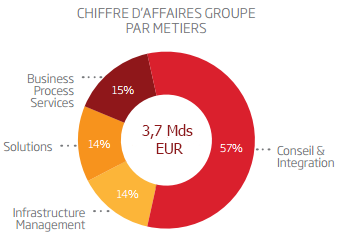
\includegraphics[scale=0.9]{images/entreprise/sopraSteriaMetiers.png}
	\centering
	\caption{Secteurs d'activités}
	\label{sopraSteriaActivites}
   \end{minipage} \hfill
   \begin{minipage}[c]{.45\linewidth}
    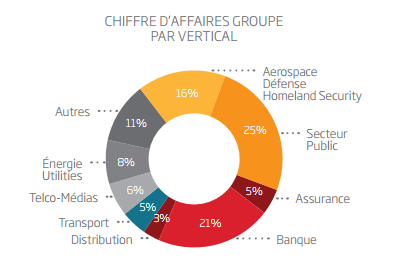
\includegraphics[scale=0.9]{images/entreprise/sopraSteriaActivites.png}
	\centering
	\caption{Répartition des activités}
	\label{sopraSteriaActivites}
   \end{minipage}
\end{figure}
		